\documentclass[english,notitlepage]{revtex4-2}  % defines the basic parameters of the document
%For preview: skriv i terminal: latexmk -pdf -pvc filnavn



% if you want a single-column, remove reprint

% allows special characters (including æøå)
\usepackage[utf8]{inputenc}
%\usepackage[english]{babel}

%% note that you may need to download some of these packages manually, it depends on your setup.
%% I recommend downloading TeXMaker, because it includes a large library of the most common packages.

\usepackage{physics,amssymb}  % mathematical symbols (physics imports amsmath)
\include{amsmath}
\usepackage{graphicx}         % include graphics such as plots
\usepackage{xcolor}           % set colors
\usepackage{hyperref}         % automagic cross-referencing (this is GODLIKE)
\usepackage{listings}         % display code
%\usepackage{subfigure}        % imports a lot of cool and useful figure commands
\usepackage{float}
%\usepackage[section]{placeins}
\usepackage{algorithm}
\usepackage[noend]{algpseudocode}
%\usepackage{subfigure}
\usepackage{tikz}
\usetikzlibrary{quantikz}
\usepackage{caption}
\usepackage{subcaption}
\usepackage{amsmath}

% defines the color of hyperref objects
% Blending two colors:  blue!80!black  =  80% blue and 20% black
\hypersetup{ % this is just my personal choice, feel free to change things
	colorlinks,
	linkcolor={red!50!black},
	citecolor={blue!50!black},
	urlcolor={blue!80!black}}

%% Defines the style of the programming listing
%% This is actually my personal template, go ahead and change stuff if you want



%% USEFUL LINKS:
%%
%%   UiO LaTeX guides:        https://www.mn.uio.no/ifi/tjenester/it/hjelp/latex/
%%   mathematics:             https://en.wikibooks.org/wiki/LaTeX/Mathematics

%%   PHYSICS !                https://mirror.hmc.edu/ctan/macros/latex/contrib/physics/physics.pdf

%%   the basics of Tikz:       https://en.wikibooks.org/wiki/LaTeX/PGF/Tikz
%%   all the colors!:          https://en.wikibooks.org/wiki/LaTeX/Colors
%%   how to draw tables:       https://en.wikibooks.org/wiki/LaTeX/Tables
%%   code listing styles:      https://en.wikibooks.org/wiki/LaTeX/Source_Code_Listings
%%   \includegraphics          https://en.wikibooks.org/wiki/LaTeX/Importing_Graphics
%%   learn more about figures  https://en.wikibooks.org/wiki/LaTeX/Floats,_Figures_and_Captions
%%   automagic bibliography:   https://en.wikibooks.org/wiki/LaTeX/Bibliography_Management  (this one is kinda difficult the first time)
%%   REVTeX Guide:             http://www.physics.csbsju.edu/370/papers/Journal_Style_Manuals/auguide4-1.pdf
%%
%%   (this document is of class "revtex4-1", the REVTeX Guide explains how the class works)


%% CREATING THE .pdf FILE USING LINUX IN THE TERMINAL
%%
%% [terminal]$ pdflatex template.tex
%%
%% Run the command twice, always.
%% If you want to use \footnote, you need to run these commands (IN THIS SPECIFIC ORDER)
%%
%% [terminal]$ pdflatex template.tex
%% [terminal]$ bibtex template
%% [terminal]$ pdflatex template.tex
%% [terminal]$ pdflatex template.tex
%%
%% Don't ask me why, I don't know.

\begin{document}
\title{Project 1}      % self-explanatory
\author{Olav K. Arnesen}          % self-explanatory
\date{\today}                             % self-explanatory
\noaffiliation                            % ignore this, but keep it.

\maketitle 

\textit{https://github.com/olavkar/fys3150/tree/main/project1}

\section*{Problem 1}
To check whether $u(x)=1-(1-e^{-10})x-e^{-100x}$ is a solution or not we insert it into the Poisson equation:
\begin{equation}
	\begin{split}	
		f(x)=&-\frac{d^2u(x)}{dx^2} \\
		=&-\frac{d^2}{dx^2}\left[1-\left(1-e^{-10}\right)x-e^{-10x}\right] \\ 
		=&-\frac{d}{dx}\left[1-e^{-10}+10e^{-10x}\right] \\
		=&100e^{-10x}
	\end{split} 
\end{equation}
which is the expected solution.

\section*{Problem 2}
Using $n=1000$ steps between $x=0$ and $x=1$ we got Fig. \ref{fig:1}.

\begin{figure}
	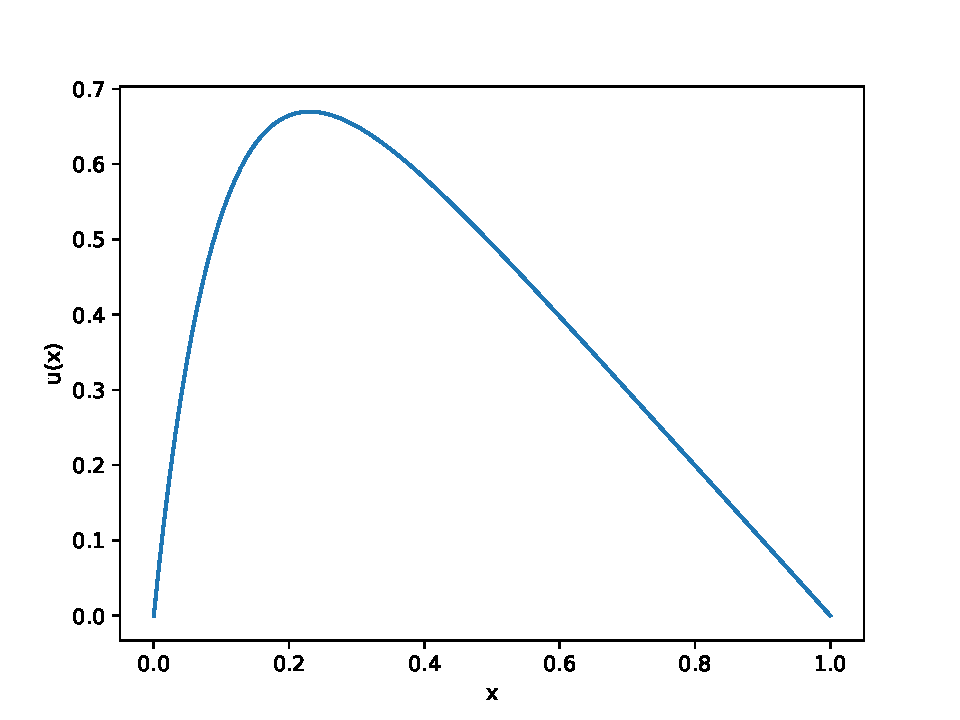
\includegraphics[scale=0.9]{imgs/problem2_output.pdf}
	\caption{The function $u(x)$ from $x=0$ to $x=1$.}
	\label{fig:1}
\end{figure}

\section*{Problem 3}
The second derivative of $u(x_i)=u_i$, where $i=1,2\ldots n$, is given numerically by
\begin{equation}
	u_i'' = \frac{u_{i+1}-2u_i+u_{i-1}}{h^2}+O(h^2) 
\end{equation}
where $h=\frac{x_{n}-x_1}{n}$ and $O(h^2)$ are all terms of order $h^2$ or higher. Inserting the Poisson equation and removing higher order terms we get the equation
\begin{equation}
	-v_{i+1}+2v_i-v_{i-1}=h^2f_i
\end{equation}
where $v_i\approx u_i$ and $f(x_i)=f_i$. We can rename $h^2f_i$ to $g_i$ to get a discretized Poission equation
\begin{equation}
	-v_{i+1}+2v_i-v_{i-1}=g_i
\end{equation}

\section*{Problem 4}
We can write out the discretized Poisson equation for all $i$:
\begin{alignat*}{8}
	i=1:&& 2&v_1&& -v_2&& + 0&& + 0&& \cdots+ 0&&+ 0&&=g_1 \\
	i=2:&& -&v_1&& +2v_2&& - v_3&& + 0&& \cdots+ 0&&+ 0&&=g_2 \\
	i=3:&& &0&& -v_2&& + 2v_3&& - v_3&& \cdots+0&&+ 0&&=g_3 \\
	&& & && && && \vdots && && && \\
	i=n:&& &0&& +0&& + 0&& +0&& \cdots-v_{n-1}&&+2v_n &&=g_n \\
\end{alignat*}
If we define two vectors $\vec{v}=(v_0, v_1,\ldots v_n)$ and $\vec{g}=(g_0, g_1,\ldots g_n)$ we can clearly see these equations can be represented by 
\begin{equation}
	\begin{pmatrix}
		2 & -1 & 0 & 0 & \ldots & 0 \\
		-1 & 2 & -1 & 0 & \ldots & 0 \\
		0 & -1 & 2 & -1 & \ldots & 0 \\
		& & \vdots & & & \\
		0 & 0 & 0 & 0 & \ldots & 2 
	\end{pmatrix}
	\begin{pmatrix}
		v_1 \\
		v_2 \\ 
		v_3 \\
		\vdots \\ 
		v_n
	\end{pmatrix}
	=
	\begin{pmatrix}
		g_1 \\
		g_2 \\ 
		g_3 \\
		\vdots \\ 
		g_n
	\end{pmatrix}
\end{equation}
where the left-hand matrix is a tri-diagonal $n\cross n$-matrix, where all elements in the main diagonal is 2 and the elements in the sub- and superdiagonal are -1. If we call the matrix \textbf{A} we can write the vector equation as 
\begin{equation}\label{eq:1}
	\textbf{A}\vec{v}=\vec{g}
\end{equation}

\section*{Problem 5}
\subsection*{a)}
$\vec{v}^*$ being a complete solution means it includes the endpoints $x=0$ and $x=1$, while $\vec{v}$ does not (though that was not obvious to me without help from a teacher). This means $m=n+2$.

\subsection*{b)}
When we solve for $\vec{v}$ we find the middle part of $\vec{v}^*$, i.e. not the endpoints. We could write $\vec{v}^*=(0, v_1, v_2,\ldots, v_n, 0)$.

\section*{Problem 6}
\subsection*{a)}
Algorithm derived in lecture on 2.09.2022.
\begin{algorithm}[H]
	\caption{Gaussian elimination}
	\begin{algorithmic}
		\State Subdiagonal: $\vec{a}=(a_2, a_3, \ldots, a_n)$
		\State Main diagonal: $\vec{b}=(b_1, b_2, \ldots, b_n)$
		\State Superdiagonal: $\vec{c}=(c_1, c_2, \ldots, c_{n-1})$
	\end{algorithmic}
	\begin{algorithmic}
		\State $\tilde{g_1}=g_1$ \Comment{Forward substitution}
		\State $\tilde{b_1}=b_1$
		\For{$i = 2, \ldots, n$}
		\State $\tilde{g_i}=g_i-\frac{a_i}{b_{i-1}}g_{i-1}$ 
		\State $\tilde{b_i}=b_i-\frac{a_i}{b_{i-1}}c_{i-1}$
		\EndFor
	\end{algorithmic}
	\begin{algorithmic}		
		\State $v_n=\frac{\tilde{g_n}}{\tilde{b_n}}$ \Comment{Back substitution}
		\For{$i = n-1, \ldots, 1$}
		\State $v_i=\frac{\tilde{g_i}-c_iv_{i+1}}{\tilde{b_i}}$
		\EndFor
	\end{algorithmic}
	\label{alg:1}
\end{algorithm}

\subsection*{b)}
The number of FLOPs from forward substitution is $(n-1)\cdot2\cdot3$, (3 in $\tilde{g_i}$, 3 in $\tilde{b_i}$, $n-1$ times). From back substitution there are $(n-1)\cdot3+1$, (3 in $v_i$, $(n-1)$ times, plus $v_n$). The total number of FLOPs is $(n-1)\cdot2\cdot3+(n-1)\cdot3+1=9n-9\approx9n$ for large $n$.

\section*{Problem 7}
\subsection*{a)}
Using the algorithm for $n=1000$ non-endpoints and plotting the results gives us Fig. \ref{fig:2}.

\begin{figure}
	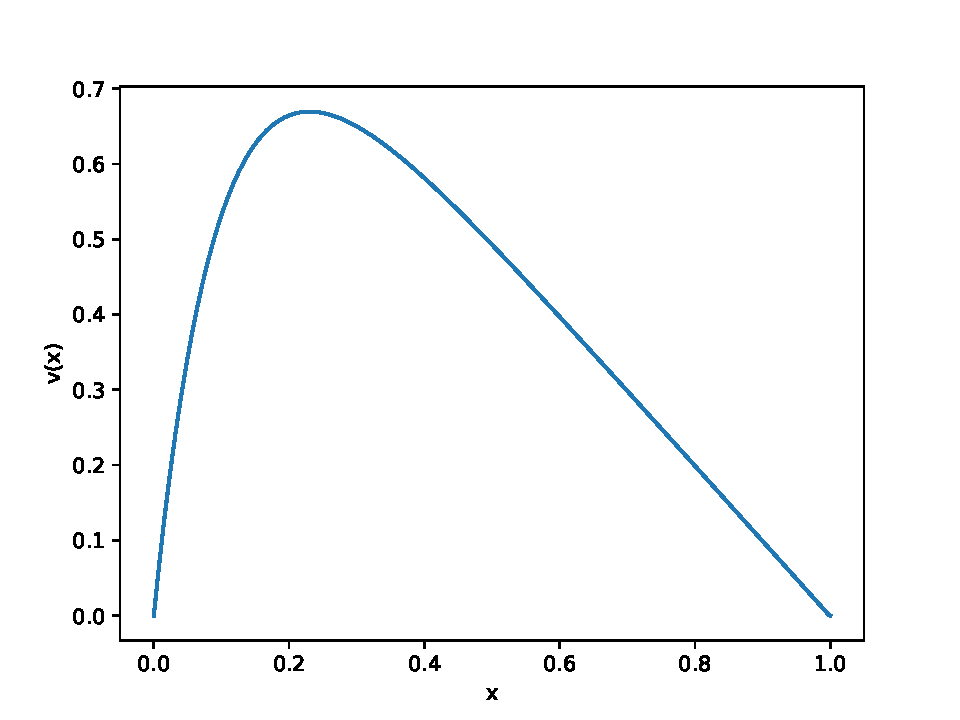
\includegraphics[scale=0.9]{imgs/problem7_output.pdf}
	\caption{The function $v(x)$ from $x=0$ to $x=1$.}
	\label{fig:2}
\end{figure}

\subsection*{b)}
For $n_{\text{steps}}\in\{10, 100, 1000\}$ we get Fig. \ref{fig:3}. Additional figures using higher $n_{\text{steps}}$ would be indistinguishable from the current ones.

\begin{figure}[h]
	\centering
	\begin{subfigure}[b]{0.45\textwidth}
		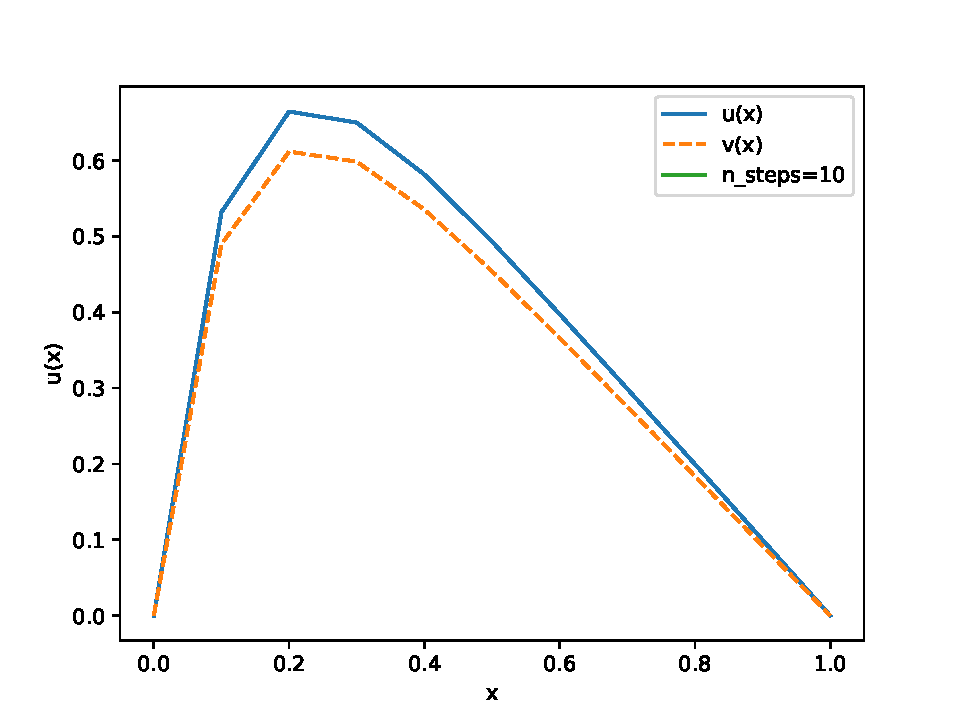
\includegraphics[scale=0.5]{imgs/problem7b_output_10.pdf}	
	\end{subfigure}
	\begin{subfigure}[b]{0.45\textwidth}
		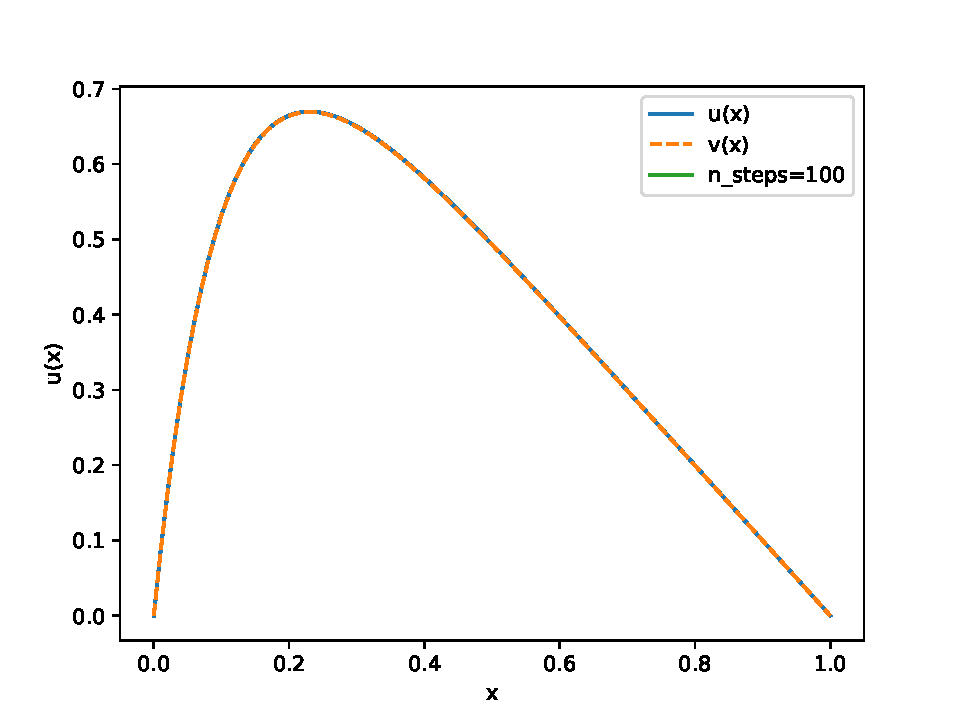
\includegraphics[scale=0.5]{imgs/problem7b_output_100.pdf}	
	\end{subfigure}	
	\begin{subfigure}[b]{0.45\textwidth}
		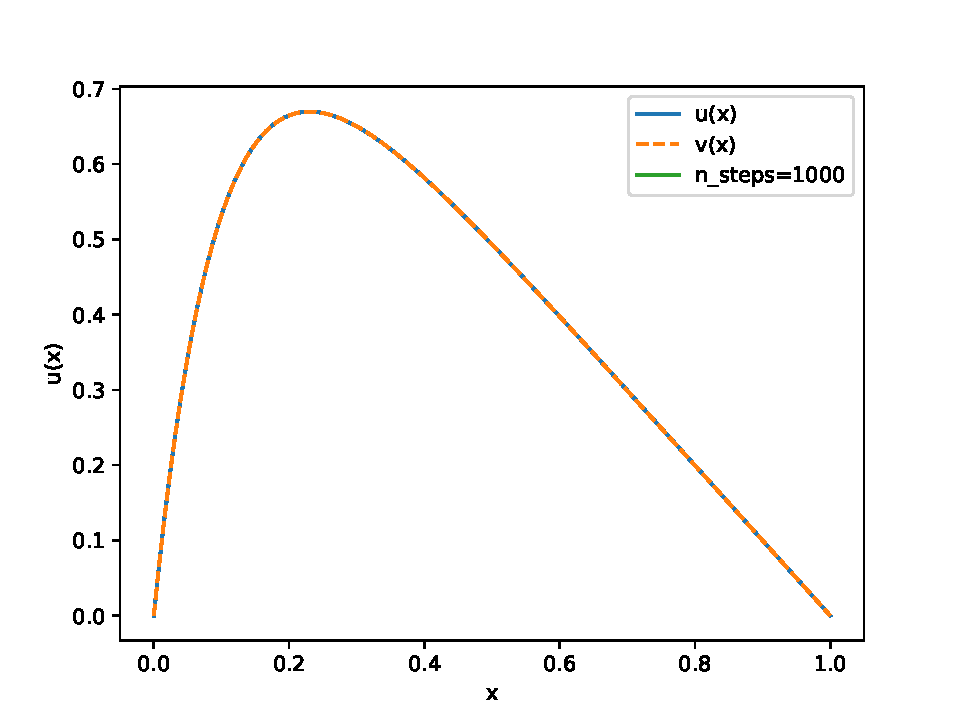
\includegraphics[scale=0.5]{imgs/problem7b_output_1000.pdf}	
	\end{subfigure}	
	\caption{$u(x)$ and $v(x)$ as functions of $x$ using $n_{\text{steps}}\in\{10, 100, 1000\}$} steps.
	\label{fig:3}
\end{figure}

\section*{Problem 8}
\subsection*{a) \& b)}
Fig. \ref{fig:4} shows the absolute and relative errors for $n_{\text{steps}}\in\{10, 100, 1000\}$.

\begin{figure}
	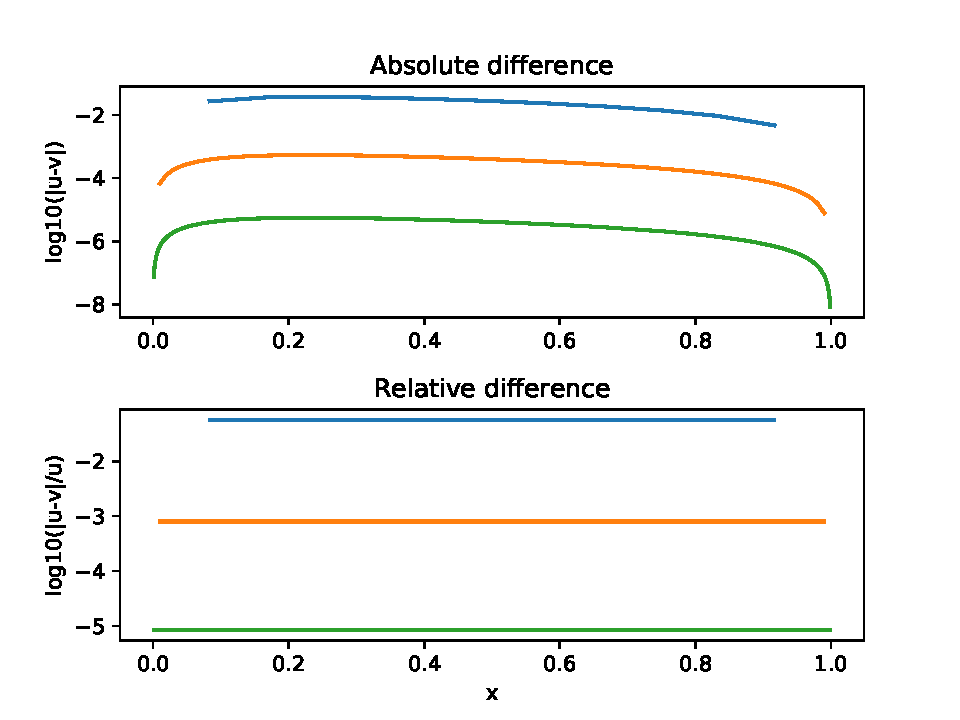
\includegraphics[scale=0.9]{imgs/problem8_output.pdf}
	\caption{$\log_{10}(|u_i-v_i|)$ and $\log_{10}(|\frac{u_i-v_i}{u_i}|)$ as functions of $x_i$. Blue corresponds to $n_{\text{steps}}=10$, orange to 100, and green to 1000 steps.}
	\label{fig:4}
\end{figure}

\subsection*{c)}
The maximum relative errors are given in table \ref{tab:1}. We can see that the relative error decreases as we go up to $10^5$ steps and increases again with additional steps. Fig. \ref{fig:5} shows that for $n_{\text{steps}}=10^7$ we get a shape (somewhat) similar to what was predicted during lecture 5, I believe. 
\begin{table}
	\centering
	\caption{Maximum relative errors}
	\begin{tabular}{c@{\hspace{1cm}} c}
		\hline
		$\log_{10}(n_{\text{steps}})$ & Maximum $\log_{10}(\epsilon_i)$ \\
		\hline
		1 & -1.25 \\
		2 &  -3.10 \\
		3 &  -5.08 \\
		4 &  -7.08 \\
		5 &  -8.84 \\
		6 &  -6.08 \\
		7 &  -5.53 \\
		\hline
	\end{tabular}\label{tab:1}
\end{table}

\begin{figure}
	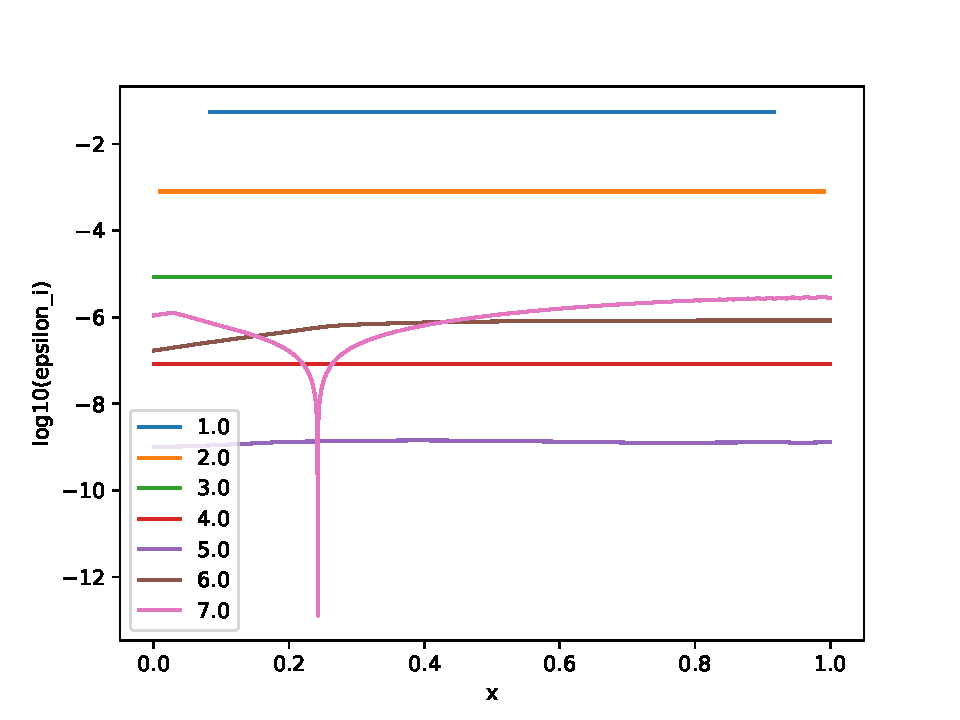
\includegraphics[scale=0.9]{imgs/problem8c_output.pdf}
	\caption{Relative error for $\log_{10}(n_{\text{steps}})\in\{1,2,3,4,5,6,7\}$.}
	\label{fig:5}
\end{figure}

\section*{Problem 9}
\subsection*{a)}
As all elements in $\vec{a}$, $\vec{b}$ and $\vec{c}$ are the same (-1, 2 and -1 respectively) we can insert these values into algorithm \ref{alg:1}. In the forward substitution we get 
\begin{equation}
	\begin{split}
		&\tilde{g_1} = g_1 \\
		&\tilde{b_1} = 2 \\
		&\tilde{g_i}=g_i+\frac{1}{2}g_{i-1} \\
		&\tilde{b_i}=2-\frac{1}{2}=\frac{3}{2}
	\end{split}
\end{equation}
In the back substitution we get 
\begin{equation}
	\begin{split}
		&v_n=\frac{2}{3}\tilde{g_n}=\frac{2}{3}(g_n+\frac{1}{2}g_{n-1}) \\
		&v_i=\frac{2}{3}(\tilde{g_i}+v_{i+1})=\frac{2}{3}(g_i+\frac{1}{2}g_{i-1}+v_{i+1}) \\
		&v_1=\frac{1}{2}(\tilde{g_1}+v_2)=\frac{1}{2}(g_1+v_2)
	\end{split}
\end{equation}
where we needed to specify $v_1$ due to $\tilde{b_1}\neq\tilde{b_i}$. Written formally we get algorithm \ref{alg:2}.
\begin{algorithm}[H]
	\caption{Special algorithm}
	\begin{algorithmic}
		\State We know all elements $g_i$.
		\State $v_n=\frac{2}{3}(g_n+\frac{1}{2}g_{n-1})$ 
		\For{$i = n-1, \ldots, 2$}
		\State $v_i=\frac{2}{3}(g_i+\frac{1}{2}g_{i-1}+v_{i+1})$
		\EndFor
		\State $v_1=\frac{1}{2}(g_1+v_2)$
	\end{algorithmic}
	\label{alg:2}
\end{algorithm}

\subsection*{b)}
The number of FLOPs in the special algorithm (not counting $\frac{1}{2}$ and $\frac{2}{3}$ as they are numbers) is $3+2+(n-2)\cdot4=4n-3\approx4n$; 3 from $v_n$, 2 from $v_1$ and 4 from $v_i$ $n-2$ times. 

\subsection*{c)}
Just look at the code. It works.

\section*{Problem 10}
\textbf{Note:} General algorithm was slightly optimized by only doing the FLOP $\frac{a_i}{b_{i-1}}$ once per $i$ instead of twice, giving a total of $8n$ FLOPs instead of $9n$.

The average time for each algorithm for the different $n_\text{steps}$ are listed in table \ref{tab:2}. We can see from the ratio of the times that the general algorithm is somewhere between 2 to 3 times slower than the special algorithm. The expected ratio would be to compare the number of FLOPs, which is $\frac{8n}{4n}=2$. 

\begin{table}
	\centering
	\caption{Average times for algorithms}
	\begin{tabular}{c c c c }
		\hline
		$\log_{10}(n_{\text{steps}})$ & Gen. Alg. [s] & Spc. Alg. [s] & Ratio \\
		\hline
		1 & $1.63\cdot10^{-6}$ & $1.17\cdot10^{-6}$ & 1.39\\
		2 & $7.10\cdot10^{-6}$ & $3.59\cdot10^{-6}$ & 1.98\\
		3 & $5.40\cdot10^{-5}$ & $1.98\cdot10^{-5}$ & 2.73\\
		4 & $2.15\cdot10^{-4}$ & $1.04\cdot10^{-4}$ & 2.07\\
		5 & $2.30\cdot10^{-3}$ & $8.99\cdot10^{-4}$ & 2.56\\
		6 & $2.37\cdot10^{-2}$ & $1.17\cdot10^{-2}$ & 2.03\\
		\hline
	\end{tabular}\label{tab:2}
\end{table}

\end{document}